% Figura cuerpo B2 (3.4.1): perturbación de demanda: la divina coincidencia
\documentclass[tikz,border=3pt]{standalone}
\usepackage[T1]{fontenc}
\usepackage[utf8]{inputenc}
\usepackage{amsmath}
\usetikzlibrary{arrows.meta,calc,positioning}
\begin{document}
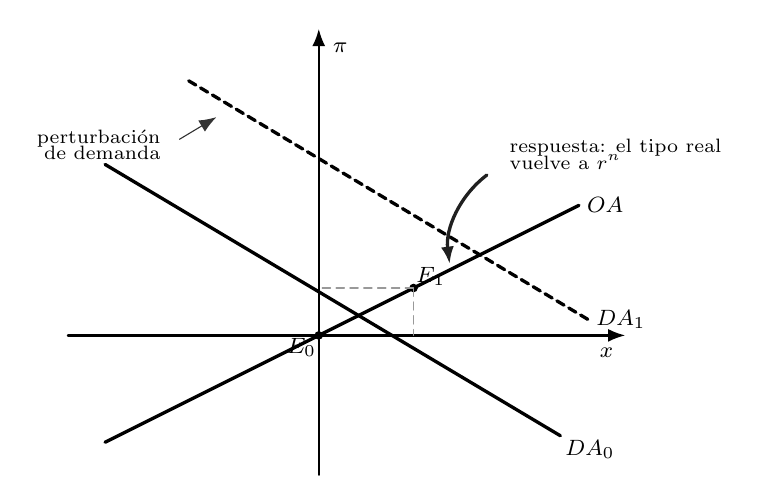
\begin{tikzpicture}[>={Latex[length=2.2mm]}, line cap=round, font=\footnotesize, scale=1.18,
  eje/.style={->, thick},
  curva/.style={very thick},
  nueva/.style={very thick, densely dashed},
  guia/.style={densely dashed, gray!80},
  pto/.style={circle, fill=black, inner sep=1.1pt}]

  \draw[eje] (-2.7,0) -- (3.3,0) node[below left=1pt]{$x$};
  \draw[eje] (0,-1.5) -- (0,3.3) node[below right=2pt]{$\pi$};

  \draw[curva] (-2.3,-1.15) -- (2.8,1.40) node[right=-1pt]{$OA$};
  \draw[curva] (-2.3,1.84) -- (2.6,-1.08) node[below right=-3pt]{$DA_{0}$};
  \draw[nueva] (-1.4,2.74) -- (2.9,0.17) node[right=-1pt]{$DA_{1}$};

  \node[pto] (E0) at (0,0) {};
  \node[below left=-2pt of E0, inner sep=1pt] {$E_{0}$};
  \node[pto] (E1) at (1.02,0.51) {};
  \node[above right=-2pt of E1, inner sep=1pt] {$E_{1}$};
  \draw[guia] (1.02,0.51) -- (1.02,0);
  \draw[guia] (1.02,0.51) -- (0,0.51);

  \draw[->, gray!40!black, shorten >=2pt, shorten <=2pt] (-1.55,2.08) -- (-1.05,2.38);
  \node[anchor=east, font=\scriptsize, align=right] at (-1.60,2.05) {perturbación\\[-2pt]de demanda};
  \draw[->, very thick, gray!25!black, shorten >=3pt, shorten <=3pt] (1.88,1.78) to[bend right=30] (1.42,0.68);
  \node[anchor=west, font=\scriptsize, align=left] at (1.95,1.95) {respuesta: el tipo real\\[-2pt]vuelve a $r^{n}$};

\end{tikzpicture}
\end{document}
